%%% %%%%%%%%%%%%%%%%%%%%%%%%%%%%%%%%%%%%%%%%%%%%%%%%%%%%%%%%%%%%%%%%%%%%%%%%%%%%
%%% %%%%%%%%%%%%%%%%%%%%%%%%%%%%%%%%%%%%%%%%%%%%%%%%%%%%%%%%%%%%%%%%%%%%%%%%%%%%

\subsubsectional{Interpretability}

There is a good deal of interest in building AI systems that are said to be {\it{interpretable}}, presumably because we believe interpretability is a property of human intelligence that we would like to emulate in the AI systems that we build and depend upon. There is a substantial literature in cognitive and behavioral neuroscience that suggests humans are not nearly as transparent and rational even at our most thoughtful and least stressed. Nick Chater captures this characteristic nicely in the title of his book, {\it{The Mind is Flat}}, in which he argues that what we generally take as cognitive depth is in fact shallow post hoc reasoning\footnote{%
%
  Nick Chater, Professor of Behavioural Science at the Warwick Business School, believes that most of what we conceive of as cognitive depth is an illusion and that actually we mostly make up things as we go along and generally post hoc. His recent book~\cite{Chater2018} entitled {\it{The Mind is Flat: The Illusion of Mental Depth and The Improvised Mind}} provides an introduction to the literature supporting this hypothesis. I don't entirely agree with him and think he overstates his case. Arguing, as Chater does, that the mind is flat basically assumes there is no {\urlh{https://en.wikipedia.org/wiki/Thinking,_Fast_and_Slow}{Type II thinking}}, only Type I~\cite{Kahneman2011}. This is like assuming that reformatting an Excel spreadsheet will always take 14 error-prone steps rather than the one step required to execute a macro that performs the reformatting flawlessly. It assumes we can't listen to a well-argued case for acting contrary to the way we've acted in the past and then successfully change our customary behavior to act in accord with the convincing argument. 

  It assumes we can't overcome our instincts and biases even if we train ourselves to recognize occasions when we might instinctively succumb to those biases and arrange things so that bells and whistles go off in our heads to remind us to sidestep the temptation. Somewhat more charitably, perhaps Chater is saying that in many contexts in which the outcome doesn't matter one way or another we allow ourselves to give into our biases \emdash{} we simply can't be bothered to think more deeply about the alternatives. Or perhaps, being less charitable to all the rest of us, Chater is saying that even in contexts that matter we can't be bothered to do the right thing \emdash{} or at least can't be bothered / aren't disciplined enough to think carefully enough to convince ourselves to do the right thing. I expect quite a number of us have the inclination and resolve to demonstrate that Chater is exaggerating his claim with respect to situations where it makes a difference.}.

If you agree with Chater's hypothesis, it would appear that by building systems modeled after the architecture of the human brain and forced to learn about the world in the same way we do, we will have to either give up on interpretability and transparency at least at the level and to the degree that some believe is necessary, or completely redesign the architectures of the current generation of artificial neural-network AI systems to operate on different principles. I believe that the demand for interpretability constitutes a double standard and is a throwback to the heyday of symbolic AI systems that are brittle in large part because unlike modern neural networks they rely upon categories with crisp boundaries and ostensibly precise, unambiguous semantic interpretations.

The programmer's apprentice is equipped with a powerful physics engine for the world in which it operates, namely the world of computer programs running on von Neumann computing architectures. This engine takes the form of an integrated development environment (IDE) specially instrumented to make it extremely easy for the assistant to explore the world of code and computation while physically manipulating the parameters of that world so as to coerce the underlying physics to yield solutions to computational problems. When it come to running code, however, the apprentice can't violate the physics of the native computing hardware.

While the interface to the IDE can be adapted to suit the needs of the apprentice, i.e., it is fully differentiable, the IDE itself and the representations that it relies upon are not differentiable and hence not amenable to adaptation via gradient descent. Moreover, the internal representations that the apprentice uses to reason about the behavior of running programs is typical of connectionist representations in that does not exhibit crisp concept boundaries or depend on immutable semantic categories. This is not really any different from the way our brains relate to the physical world in which we struggle to survive. However, the world of the apprentice is in many ways even less forgiving than the world in which we inhabit.

The language interface that determines how the programmer and apprentice relate to one another and collaborate to solve problems is patterned after human-to-human interaction and hence is subject to all the advantages and inadequacies that we observe in human-to-human collaboration and the struggle that software engineers face in translating human needs and aspirations into reliable products and computing platforms. One solution to the problem of interpretability is to design failsafe systems that limit what the non-differentiable components are capable of doing just as we attempt to build control systems that limit what their human operators are able to do.

By the way, I'm confident that the sort of digital assistants based upon what we know about human brains implemented as artificial neural networks will be able to provide post hoc interpretations for their actions. However, if we do a good job of capturing human reasoning, I wouldn't give those interpretations any more credence than I do humans, since the AI systems will be learning their tricks from listening to humans. Perhaps if we want systems that behave more like us in those respects we admire but better in those that we abhor, then we will have to design very different ways of training these systems than we use to educate our own children and not expose them to the sort of unscrupulous politicians we seem to elect or the entrepreneurs and businessmen whose successes and excesses our youth seek to emulate.

%%% %%%%%%%%%%%%%%%%%%%%%%%%%%%%%%%%%%%%%%%%%%%%%%%%%%%%%%%%%%%%%%%%%%%%%%%%%%%%
%%% %%%%%%%%%%%%%%%%%%%%%%%%%%%%%%%%%%%%%%%%%%%%%%%%%%%%%%%%%%%%%%%%%%%%%%%%%%%% 

\section{Introduction}
\section{Inspiration}
\section{Foundation}
\section{Representation}
\section{Communication}
\section{Interaction}
\section{Production}
\section{Generation}
\section{Synthesis}

%%% %%%%%%%%%%%%%%%%%%%%%%%%%%%%%%%%%%%%%%%%%%%%%%%%%%%%%%%%%%%%%%%%%%%%%%%%%%%%

\section{Introduction: The Programmer's Apprentice}  %%% https://en.wikipedia.org/wiki/Knowledge_Based_Software_Assistant
\section{Representation: Cognitive Neurosciences}    %%% https://en.wikipedia.org/wiki/Knowledge_representation_and_reasoning
\section{Interaction: Natural Language Processing}    %%% https://en.wikipedia.org/wiki/Natural_language_processing
\section{Generation: Automated Code Synthesis}      %%% https://en.wikipedia.org/wiki/Automatic_programming

%%% %%%%%%%%%%%%%%%%%%%%%%%%%%%%%%%%%%%%%%%%%%%%%%%%%%%%%%%%%%%%%%%%%%%%%%%%%%%%

\section{Knowledge Representation} https://en.wikipedia.org/wiki/Knowledge_representation_and_reasoning ~\cite{Brachmanetal2004}
\section{The Cognitive Neurosciences} https://en.wikipedia.org/wiki/Cognitive_neuroscience ~\cite{Gazzaniga2009}

%%% %%%%%%%%%%%%%%%%%%%%%%%%%%%%%%%%%%%%%%%%%%%%%%%%%%%%%%%%%%%%%%%%%%%%%%%%%%%%
%%% %%%%%%%%%%%%%%%%%%%%%%%%%%%%%%%%%%%%%%%%%%%%%%%%%%%%%%%%%%%%%%%%%%%%%%%%%%%% 

This particular section concerns the topic of {\urlh{https://en.wikipedia.org/wiki/Knowledge_representation_and_reasoning}{knowledge representation}}~\cite{Brachmanetal2004} as it applies to the programmer's apprentice problem and emphasises contributions from the {\urlh{https://en.wikipedia.org/wiki/Cognitive_neuroscience}{cognitive neurosciences}}~\cite{Gazzaniga2009} as they apply to modeling how information is represented in human-inspired cognitive architectures and connectionist models in particular\footnote{%
%
The phrases {\urlh{https://en.wikipedia.org/wiki/Knowledge_representation_and_reasoning}{Knowledge Representation}}~\cite{Brachmanetal2004} and {\urlh{https://en.wikipedia.org/wiki/Cognitive_neuroscience}{Cognitive Neuroscience}}~\cite{Gazzaniga2009} refer to important long-standing areas of study, each with their respective academic departments, national and international conferences and large numbers of advocates and adepts. Mentioning them both in the same breath could be orthodoxy or heresy depending on the context and the company you keep, but both disciplines \emdash{} it could be argued that each one of the two phrases might better be described as a constellation of specialized disciplines\footnote{%
%
  The phrase {\urlh{https://en.wikipedia.org/wiki/Knowledge_representation_and_reasoning}{Knowledge Representation}} seems so dated that it must be back in vogue again. It's interesting to think about the evolution of our thinking about representation as chronicled in the names of major technical conferences relating to artificial intelligence. By 1990, the major national and international AI conferences, including the {\urlh{http://www.aaai.org/Conferences/conferences.php}{National Conference on Artificial Intelligence}} \emdash{} I co-chaired the conference in 1991 when it was held in Anaheim, California \emdash{} and the {\urlh{https://ijcai.org/}{International Joint Conference on Artificial Intelligence}} \emdash{} I co-chaired IJCAI-99 held in Stockholm, were getting so large and were receiving so many submissions that first satellite and then independent conferences began springing up to cater to special interests including researchers interested in representation. For example, Ronald Brachman, Hector Levesque and Raymond Reiter co-chaired the first {\urlh{http://www.kr.org/index.php}{International Conference on Knowledge Representation and Reasoning}} (KR-89) in 1989. Then Usama Fayyad and Ramasamy Uthurusamy chaired the first {\urlh{https://www.aaai.org/Press/Proceedings/kdd95.php}{International Conference on Knowledge Discovery and Data Mining}} (KDD-95) in 1995. More recently Yoshua Bengio and Yann LeCun chaired the first {\urlh{International Conference on Learning Representations}{International Conference on Learning Representations}} (ICLR-13) in 2013. We might extrapolate the trend and imagine Vinod Khosla, Ray Kurzweil, Elon Musk, Peter Thiel and Mark Zuckerberg will co-chair the first {\urlh{https://www.santafe.edu/research/initiatives/interplanetary-project}{Interplanetary Conference on Instantaneous Thought and Infinitely Extensible Memory}} (ITEM-37) in 2037.} 
%
\emdash{} have made major contributions to our understanding of intelligence both biological and artificial. Together cognitive neurosciences make up a small but active contingent within the larger population of scientists who consider themselves part of neuroscience including anatomical, behavioral, cellular, cognitive, computational, developmental, genetic, molecular, pharmacological, physiological, psychological and systems neuroscience focusing on neural circuits and their function.}

%%% %%%%%%%%%%%%%%%%%%%%%%%%%%%%%%%%%%%%%%%%%%%%%%%%%%%%%%%%%%%%%%%%%%%%%%%%%%%%

{{\urlh{https://web.stanford.edu/class/cs379c/calendar_invited_talks/lectures/04/05/slides/index.html#CS379C_INTRODUCTORY_LECTURE_2_SLIDE_02}{Slide~2}}} %%% relevant anatomy of the brain\\
{{\urlh{https://web.stanford.edu/class/cs379c/calendar_invited_talks/lectures/04/05/slides/index.html#CS379C_INTRODUCTORY_LECTURE_2_SLIDE_03}{Slide~3}}} %%% schema theory, global workspace theory\\
{{\urlh{https://web.stanford.edu/class/cs379c/calendar_invited_talks/lectures/04/05/slides/index.html#CS379C_INTRODUCTORY_LECTURE_2_SLIDE_05}{Slide~5}}} %%% global workspace theory\\
{{\urlh{https://web.stanford.edu/class/cs379c/calendar_invited_talks/lectures/04/05/slides/index.html#CS379C_INTRODUCTORY_LECTURE_2_SLIDE_06}{Slide~6}}} %%% basic artificial neural network architecture\\
{{\urlh{https://web.stanford.edu/class/cs379c/calendar_invited_talks/lectures/04/05/slides/index.html#CS379C_INTRODUCTORY_LECTURE_2_SLIDE_07}{Slide~7}}} %%% programmer's apprentice network architecture\\
{{\urlh{https://web.stanford.edu/class/cs379c/calendar_invited_talks/lectures/04/05/slides/index.html#CS379C_INTRODUCTORY_LECTURE_2_SLIDE_10}{Slide~10}}} %%% somatosensory and primary motor cortex\\
{{\urlh{https://web.stanford.edu/class/cs379c/calendar_invited_talks/lectures/04/05/slides/index.html#CS379C_INTRODUCTORY_LECTURE_2_SLIDE_11}{Slide~11}}} %%% integrated development environment\\
{{\urlh{https://web.stanford.edu/class/cs379c/calendar_invited_talks/lectures/04/05/slides/index.html#CS379C_INTRODUCTORY_LECTURE_2_SLIDE_13}{Slide~13}}} %%% entorhinal cortex and episodic memory\\
{{\urlh{https://web.stanford.edu/class/cs379c/calendar_invited_talks/lectures/04/05/slides/index.html#CS379C_INTRODUCTORY_LECTURE_2_SLIDE_14}{Slide~14}}} %%% complementary learning and the hippocampus\\
{{\urlh{https://web.stanford.edu/class/cs379c/calendar_invited_talks/lectures/04/05/slides/index.html#CS379C_INTRODUCTORY_LECTURE_2_SLIDE_15}{Slide~15}}} %%% machine theory of mind model\\

%%% %%%%%%%%%%%%%%%%%%%%%%%%%%%%%%%%%%%%%%%%%%%%%%%%%%%%%%%%%%%%%%%%%%%%%%%%%%%%

%%% GLOVE .... https://nlp.stanford.edu/projects/glove/

GloVe is an unsupervised learning algorithm for obtaining vector representations for words. Training is performed on aggregated global word-word co-occurrence statistics from a corpus, and the resulting representations showcase interesting linear substructures of the word vector space.

%%% GAIL .... https://arxiv.org/abs/1606.03476

We propose a new general framework for directly extracting a policy from data as if it were obtained by reinforcement learning following inverse reinforcement learning. We show that a certain instantiation of our framework draws an analogy between imitation learning and generative adversarial networks, from which we derive a model-free imitation learning algorithm that obtains significant performance gains over existing model-free methods in imitating complex behaviors in large, high-dimensional environments.

%%% The Jargon of the New, Deeper Freemasonry

The jargon of modern (deep) neural networks is like the argot of a new Fremasonry that has hardly begun to lay the foundations for the restoration of the connectionist temple. Terms like attention, consciousness, imagination, rewards and reinforcement get bandied about as if deeply descriptive of the architectures they are invoked to describe. The odd thing is that on more than one occasion I have found they reveal more than they obfuscate. Still, the learning curve is steep, and the mountain is constantly moving.

%%% %%%%%%%%%%%%%%%%%%%%%%%%%%%%%%%%%%%%%%%%%%%%%%%%%%%%%%%%%%%%%%%%%%%%%%%%%%%%

\rawhtml
<a name="introduction_and_high_level_content"></a>
\endrawhtml
\subsection*{Introduction}

%%% %%%%%%%%%%%%%%%%%%%%%%%%%%%%%%%%%%%%%%%%%%%%%%%%%%%%%%%%%%%%%%%%%%%%%%%%%%%%

%%% %%%%%%%%%%%%%%%%%%%%%%%%%%%%%%%%%%%%%%%%%%%%%%%%%%%%%%%%%%%%%%%%%%%%%%%%%%%%

\rawhtml
<a name="foundation_cognitive_neuroscience"></a>
\endrawhtml
\subsection*{Foundations}

%%% %%%%%%%%%%%%%%%%%%%%%%%%%%%%%%%%%%%%%%%%%%%%%%%%%%%%%%%%%%%%%%%%%%%%%%%%%%%%

%%% %%%%%%%%%%%%%%%%%%%%%%%%%%%%%%%%%%%%%%%%%%%%%%%%%%%%%%%%%%%%%%%%%%%%%%%%%%%%

\subsubsection*{Resources}

Michael Graziano's {\urlh{https://web.stanford.edu/class/cs379c/calendar_invited_talks/lectures/04/10/videos/Michael_Graziano_CS379C_04-10-18.mp4}{presentation}} on machines that incorporate an internal model of what consciousness is and attribute that model to themselves and others to make predictions about human behavior~\cite{GrazianoFiRAI-17}\footnote{%
%
  The abstract for Graziano~\cite{GrazianoFiRAI-17}:
%
  \begin{quotation}
%
   The purpose of the attention schema theory is to explain how an information-processing device, the brain, arrives at the claim that it possesses a non-physical, subjective awareness, and assigns a high degree of certainty to that extraordinary claim. The theory does not address how the brain might actually possess a non-physical essence. It is not a theory that deals in the non-physical. It is about the computations that cause a machine to make a claim and to assign a high degree of certainty to the claim. The theory is offered as a possible starting point for building artificial consciousness. Given current technology, it should be possible to build a machine that contains a rich internal model of what consciousness is, attributes that property of consciousness to itself and to the people it interacts with, and uses that attribution to make predictions about human behavior. Such a machine would “believe” it is conscious and act like it is conscious, in the same sense that the human machine believes and acts.
%
  \end{quotation}}.

Randall O'Reilly's {\urlh{https://web.stanford.edu/class/cs379c/calendar_invited_talks/lectures/04/12/videos/Randall_OReilly_CS379C_04-12-18.mp4}{presentation}} on learning mechanisms that rely on a computational model of the prefrontal cortex to control both itself and other brain areas in a strategic, task-appropriate manner~\cite{OReillyandFrankNC-06}\footnote{%
%
  The abstract for O'Reilly and Frank~\cite{OReillyandFrankNC-06}:
%
  \begin{quotation}
%
   The prefrontal cortex has long been thought to subserve both working memory (the holding of information online for processing) and executive functions (deciding how to manipulate working memory and perform processing). Although many computational models of working memory have been developed, the mechanistic basis of executive function remains elusive, often amounting to a homunculus. This article presents an attempt to deconstruct this homunculus through powerful learning mechanisms that allow a computational model of the prefrontal cortex to control both itself and other brain areas in a strategic, task-appropriate manner. These learning mechanisms are based on subcortical structures in the midbrain, basal ganglia, and amygdala, which together form an actor-critic architecture. The critic system learns which prefrontal representations are task relevant and trains the actor, which in turn provides a dynamic gating mechanism for controlling working memory updating. Computationally, the learning mechanism is designed to simultaneously solve the temporal and structural credit assignment problems.
%
  \end{quotation}}.

Jay McClelland's {\urlh{https://web.stanford.edu/class/cs379c/calendar_invited_talks/lectures/04/19/slides/Jay_McClelland_CS379C_04-19-18.pdf}{presentation}} on complementary learning systems that avoid catastrophic forgetting and support the stable learning of new knowledge and learning with imbalanced class labels~\cite{SprechmannetalICLR-18}\footnote{%
%
  The abstract for Sprechmann~\etal{}~\cite{SprechmannetalICLR-18}:
%
  \begin{quotation}
%
   Deep neural networks have excelled on a wide range of problems, from vision to language and game playing. Neural networks very gradually incorporate information into weights as they process data, requiring very low learning rates. If the training distribution shifts, the network is slow to adapt, and when it does adapt, it typically performs badly on the training distribution before the shift. Our method, Memory-based Parameter Adaptation, stores examples in memory and then uses a context-based lookup to directly modify the weights of a neural network. Much higher learning rates can be used for this local adaptation, reneging the need for many iterations over similar data before good predictions can be made. As our method is memory-based, it alleviates several shortcomings of neural networks, such as catastrophic forgetting, fast, stable acquisition of new knowledge, learning with an imbalanced class labels, and fast learning during evaluation. We demonstrate this on a range of supervised tasks: large-scale image classification and language modelling.
%
  \end{quotation}}.

Matt Botvinick's {\urlh{https://web.stanford.edu/class/cs379c/calendar_invited_talks/lectures/04/26/slides/Matt_Botvinick_CS379C_04-26-18.pdf}{presentation}} describing a new model of reward-based learning in which a traditional dopamine system trains the prefrontal cortex to operate as its own free-standing learning system~\cite{WangetalNATURE-NEUROSCIENCE-18}\footnote{%
%
  The abstract for Wang~\etal{}~\cite{WangetalNATURE-NEUROSCIENCE-18}:
%
  \begin{quotation}
%
   Over the past 20 years, neuroscience research on reward-based learning has converged on a canonical model, under which the neurotransmitter dopamine stamps in associations between situations, actions and rewards by modulating the strength of synaptic connections between neurons. However, a growing number of recent findings have placed this standard model under strain. We now draw on recent advances in artificial intelligence to introduce a new theory of reward-based learning. Here, the dopamine system trains another part of the brain, the prefrontal cortex, to operate as its own free-standing learning system. This new perspective accommodates the findings that motivated the standard model, but also deals gracefully with a wider range of observations, providing a fresh foundation for future research.
%
  \end{quotation}}.

%%% %%%%%%%%%%%%%%%%%%%%%%%%%%%%%%%%%%%%%%%%%%%%%%%%%%%%%%%%%%%%%%%%%%%%%%%%%%%%

%%% %%%%%%%%%%%%%%%%%%%%%%%%%%%%%%%%%%%%%%%%%%%%%%%%%%%%%%%%%%%%%%%%%%%%%%%%%%%%

\rawhtml
<a name="collabration_communication_value"></a>
\endrawhtml
\subsection*{Interactions}

%%% %%%%%%%%%%%%%%%%%%%%%%%%%%%%%%%%%%%%%%%%%%%%%%%%%%%%%%%%%%%%%%%%%%%%%%%%%%%%

\subsubsection*{Resources}

%%% Botvinick~\cite{WangetalBIORXIV-18} prefrontal cortex as meta learning system
%%% Rabinowitz~\etal{}~\cite{RabinowitzetalCoRR-18} theory of mind reasoning
%%% Guez~\etal{}~\cite{GuezetalCoRR-18} Monte Carlo tree search 
%%% Hamrick~\etal{}~\cite{HamricketalCoRR-17} imagination-based optimization
%%% Pascanu~\etal{}~\cite{PascanuetalCoRR-17} imagination-based planning
%%% Pritzel~\etal{}~\cite{PritzeletalCoRR-17} neural episodic control
%%% Wayne~\etal{}~\cite{WayneetalCoRR-18} unsupervised predictive memory

Neil Rabinowitz's {\urlh{https://web.stanford.edu/class/cs379c/calendar_invited_talks/lectures/04/17/slides/Neil_Rabinowitz_CS379C_04-17-18.pdf}{presentation}} on learning a machine theory-of-mind model that relies on meta-learning to build mental models of the agents that it encounters from observations of their behaviour alone~\cite{RabinowitzetalCoRR-18}\footnote{%
%
  The abstract for Rabinowitz~\etal{}~\cite{RabinowitzetalCoRR-18}:
%
  \begin{quotation}
%
    Theory of mind (ToM; Premack and Woodruff, 1978) broadly refers to humans' ability to represent the mental states of others, including their desires, beliefs, and intentions. We propose to train a machine to build such models too. We design a Theory of Mind neural network \emdash{} a ToMnet \emdash{} which uses meta-learning to build models of the agents it encounters, from observations of their behaviour alone. Through this process, it acquires a strong prior model for agents' behaviour, as well as the ability to bootstrap to richer predictions about agents' characteristics and mental states using only a small number of behavioural observations. We apply the ToMnet to agents behaving in simple gridworld environments, showing that it learns to model random, algorithmic, and deep reinforcement learning agents from varied populations, and that it passes classic ToM tasks such as the "Sally-Anne" test (Wimmer and Perner, 1983; Baron-Cohen et al., 1985) of recognising that others can hold false beliefs about the world. We argue that this system \emdash{} which autonomously learns how to model other agents in its world \emdash{} is an important step forward for developing multi-agent AI systems, for building intermediating technology for machine-human interaction, and for advancing the progress on interpretable AI.
%
\end{quotation}}.

Greg Wayne's {\urlh{https://web.stanford.edu/class/cs379c/calendar_invited_talks/lectures/05/03/slides/Greg_Wayne_CS379C_05-03-18.pdf}{presentation}} on {\tt{MERLIN}} a method for prediction in environments corresponding to partially observable Markov decision processes in which memory formation is guided by predictive modeling~\cite{WayneetalCoRR-18}\footnote{%
%
  The abstract for Wayne~\etal{}~\cite{WayneetalCoRR-18}:
%
  \begin{quotation}
%
    Animals execute goal-directed behaviours despite the limited range and scope of their sensors. To cope, they explore environments and store memories maintaining estimates of important information that is not presently available. Recently, progress has been made with artificial intelligence (AI) agents that learn to perform tasks from sensory input, even at a human level, by merging reinforcement learning (RL) algorithms with deep neural networks, and the excitement surrounding these results has led to the pursuit of related ideas as explanations of non-human animal learning. However, we demonstrate that contemporary RL algorithms struggle to solve simple tasks when enough information is concealed from the sensors of the agent, a property called "partial observability". An obvious requirement for handling partially observed tasks is access to extensive memory, but we show memory is not enough; it is critical that the right information be stored in the right format. We develop a model, the Memory, RL, and Inference Network (MERLIN), in which memory formation is guided by a process of predictive modeling. MERLIN facilitates the solution of tasks in 3D virtual reality environments for which partial observability is severe and memories must be maintained over long durations. Our model demonstrates a single learning agent architecture that can solve canonical behavioural tasks in psychology and neurobiology without strong simplifying assumptions about the dimensionality of sensory input or the duration of experiences.
%
  \end{quotation}}.

Oriol Vinyals' {\urlh{https://web.stanford.edu/class/cs379c/calendar_invited_talks/lectures/05/10/slides/Oriol_Vinyals_CS379C_05-10-18.pdf}{presentation}} on an approach for model-based plan construction, evaluation and execution applied to sequential decision making problems relying on a method of imagination-based forecasting~\cite{PascanuetalCoRR-17}\footnote{%
%
  The abstract for Pascanu~\etal{}~\cite{PascanuetalCoRR-17}:
%
  \begin{quotation}
%
   Conventional wisdom holds that model-based planning is a powerful approach to sequential decision-making. It is often very challenging in practice, however, because while a model can be used to evaluate a plan, it does not prescribe how to construct a plan. Here we introduce the "Imagination-based Planner", the first model-based, sequential decision-making agent that can learn to construct, evaluate, and execute plans. Before any action, it can perform a variable number of imagination steps, which involve proposing an imagined action and evaluating it with its model-based imagination. All imagined actions and outcomes are aggregated, iteratively, into a "plan context" which conditions future real and imagined actions. The agent can even decide how to imagine: testing out alternative imagined actions, chaining sequences of actions together, or building a more complex "imagination tree" by navigating flexibly among the previously imagined states using a learned policy. And our agent can learn to plan economically, jointly optimizing for external rewards and computational costs associated with using its imagination. We show that our architecture can learn to solve a challenging continuous control problem, and also learn elaborate planning strategies in a discrete maze-solving task. Our work opens a new direction toward learning the components of a model-based planning system and how to use them.  
%
  \end{quotation}}.

Devi Parikh's {\urlh{https://web.stanford.edu/class/cs379c/calendar_invited_talks/lectures/05/22/index.html}{public lectures}} on learning to conduct meaningful dialog with humans in natural, conversational language by grounding the conversation in shared visual experience, inferring its context from history~\cite{DasetalCVPR-17}\footnote{%
%
  The abstract for Das~\etal{}~\cite{DasetalCVPR-17}:
%
  \begin{quotation}
%
    We introduce the task of Visual Dialog, which requires an AI agent to hold a meaningful dialog with humans in natural, conversational language about visual content. Specifically, given an image, a dialog history, and a question about the image, the agent has to ground the question in the image, infer its context from history, and answer the question accurately. Visual Dialog is disentangled enough from a specific downstream task so as to serve as a general test of machine intelligence, while being grounded in vision enough to allow objective evaluation of individual responses and benchmark progress. We develop a novel two-person chat data-collection protocol to curate a large-scale Visual Dialog dataset (VisDial). VisDial v0.9 has been released and contains 1 dialog with 10 question-answer pairs on \hmapprox{}120k images from COCO, with a total of \hmapprox{}1.2M dialog question-answer pairs. We introduce a family of neural encoder-decoder models for Visual Dialog with 3 encoders \emdash{} Late Fusion, Hierarchical Recurrent Encoder and Memory Network \emdash{} and 2 decoders (generative and discriminative), which outperform a number of sophisticated baselines. We propose a retrieval-based evaluation protocol for Visual Dialog where the AI agent is asked to sort a set of candidate answers and evaluated on metrics such as mean-reciprocal-rank of human response. We quantify gap between machine and human performance on the Visual Dialog task via human studies. Our dataset, code, trained models and visual chatbot are available {\urlh{https://visualdialog.org/}{here}}.
%
  \end{quotation}}.

%%% %%%%%%%%%%%%%%%%%%%%%%%%%%%%%%%%%%%%%%%%%%%%%%%%%%%%%%%%%%%%%%%%%%%%%%%%%%%%

%%% %%%%%%%%%%%%%%%%%%%%%%%%%%%%%%%%%%%%%%%%%%%%%%%%%%%%%%%%%%%%%%%%%%%%%%%%%%%%

\rawhtml
<a name="production_code_program_synthesis
\endrawhtml
\subsection*{Production}

%%% %%%%%%%%%%%%%%%%%%%%%%%%%%%%%%%%%%%%%%%%%%%%%%%%%%%%%%%%%%%%%%%%%%%%%%%%%%%%

\subsubsection*{Resources}

Daniel Abolafia's {\urlh{https://web.stanford.edu/class/cs379c/calendar_invited_talks/lectures/04/24/slides/Daniel_Abolafia_CS379C_04-24-18.pdf}{presentation}} on iterative optimization for program synthesis in the presence of a reward function over the output of programs, where the goal is to find programs with maximal rewards~\cite{AbolafiaetalCoRR-18}\footnote{%
%
  The abstract for Abolafia~\etal{}~\cite{AbolafiaetalCoRR-18}:
%
  \begin{quotation}
%
    We consider the task of program synthesis in the presence of a reward function over the output of programs, where the goal is to find programs with maximal rewards. We employ an iterative optimization scheme, where we train an RNN on a dataset of K best programs from a priority queue of the generated programs so far. Then, we synthesize new programs and add them to the priority queue by sampling from the RNN. We benchmark our algorithm, called priority queue training (or PQT), against genetic algorithm and reinforcement learning baselines on a simple but expressive Turing complete programming language called BF. Our experimental results show that our simple PQT algorithm significantly outperforms the baselines. By adding a program length penalty to the reward function, we are able to synthesize short, human readable programs.
%
  \end{quotation}}.

Graham Neubig's {\urlh{https://web.stanford.edu/class/cs379c/calendar_invited_talks/lectures/05/01/slides/Graham_Neubig_CS379C_05-01-18.pdf}{presentation}} on a novel neural architecture for parsing natural language descriptions into source code powered by a grammar model to explicitly capture the target syntax as prior knowledge~\cite{YinandNeubigACL-17}\footnote{%
%
  The abstract for Yin and Neubig~\cite{YinandNeubigACL-17}:
%
  \begin{quotation}
%
    We consider the problem of parsing natural language descriptions into source code written in a general-purpose programming language like Python. Existing data-driven methods treat this problem as a language generation task without considering the underlying syntax of the target programming language. Informed by previous work in semantic parsing, in this paper we propose a novel neural architecture powered by a grammar model to explicitly capture the target syntax as prior knowledge. Experiments find this an effective way to scale up to generation of complex programs from natural language descriptions, achieving state-of-the-art results that well outperform previous code generation and semantic parsing approaches.
%
  \end{quotation}}.

Rishabh Singh's {\urlh{https://web.stanford.edu/class/cs379c/calendar_invited_talks/lectures/05/24/videos/Rishabh_Singh_CS379C_05-24-18.mp4}{presentation}} on using a strong statistical model for semantic code repair to predict bug locations and exact fixes without access to information about the intended correct behavior of the program.~\cite{DevlinetalICLR-18}\footnote{%
%
  The abstract for Devlin~\etal{}~\cite{DevlinetalICLR-18}:
%
  \begin{quotation}
%
    We study the problem of semantic code repair, which can be broadly defined as automatically fixing non-syntactic bugs in source code. The majority of past work in semantic code repair assumed access to unit tests against which candidate repairs could be validated. In contrast, the goal here is to develop a strong statistical model to accurately predict both bug locations and exact fixes without access to information about the intended correct behavior of the program. Achieving such a goal requires a robust contextual repair model, which we train on a large corpus of real-world source code that has been augmented with synthetically injected bugs. Our framework adopts a two-stage approach where first a large set of repair candidates are generated by rule-based processors, and then these candidates are scored by a statistical model using a novel neural network architecture which we refer to as Share, Specialize, and Compete. Specifically, the architecture (1) generates a  shared encoding of the source code using an RNN over the abstract syntax tree, (2) scores each candidate repair using specialized network modules, and (3) then normalizes these scores together so they can compete against one another in comparable probability space. We evaluate our model on a real-world test set gathered from GitHub containing four common categories of bugs. Our model is able to predict the exact correct repair 41\% of the time with a single guess, compared to 13\% accuracy for an attentional sequence-to-sequence model.
%
  \end{quotation}}.

Dawn Song and Xinyun Chen's {\urlh{https://web.stanford.edu/class/cs379c/calendar_invited_talks/lectures/05/31/videos/Dawn_Song_CS379C_05-31-18.mp4}{presentation}} on program synthesis from input-output examples, tree-to-tree neural networks for program translation, and attention for program synthesis from natural lanquage descriptions~\cite{ChenetalICLR-18b}\footnote{%
%
  The abstract for Chen~\etal{}~\cite{ChenetalICLR-18b}:
%
  \begin{quotation}
%
    Program translation is an important tool to migrate legacy code in one language into an ecosystem built in a different language. In this work, we are the first to consider employing deep neural networks toward tackling this problem. We observe that program translation is a modular procedure, in which a sub-tree of the source tree is translated into the corresponding target sub-tree at each step. To capture this intuition, we design a tree-to-tree neural network as an encoder-decoder architecture to translate a source tree into a target one. Meanwhile, we develop an attention mechanism for the tree-to-tree model, so that when the decoder expands one non-terminal in the target tree, the attention mechanism locates the corresponding sub-tree in the source tree to guide the expansion of the decoder. We evaluate the program translation capability of our tree-to-tree model against several state-of-the-art approaches. Compared against other neural translation models, we observe that our approach is consistently better than the baselines with a margin of up to 15 points. Further, our approach can improve the previous state-of-the-art program translation approaches by a margin of 20 points on the translation of real-world projects.
%
  \end{quotation}}.

%%% %%%%%%%%%%%%%%%%%%%%%%%%%%%%%%%%%%%%%%%%%%%%%%%%%%%%%%%%%%%%%%%%%%%%%%%%%%%%

%%% %%%%%%%%%%%%%%%%%%%%%%%%%%%%%%%%%%%%%%%%%%%%%%%%%%%%%%%%%%%%%%%%%%%%%%%%%%%% 
%%% %%%%%%%%%%%%%%%%%%%%%%%%%%%%%%%%%%%%%%%%%%%%%%%%%%%%%%%%%%%%%%%%%%%%%%%%%%%% 

This document is not intended to provide the reader with a short course in cognitive science, artificial intelligence, natural language processing, machine learning, artificial neural networks, or automated code synthesis / automatic inductive programming, and is certainly not intended to cover all these disciplines in any but the most cursory of detail. The primary goal is to explore the possibility of building digital assistants that considerably extend our ability to solve complex engineering problems with a emphasis here on software engineering. A secondary goal is to explain how the field of neuroscience is helping to achieve our primary goal. 

The fields of cognitive and systems neuroscience are playing an important role in directing and accelerating research on artificial neural network systems. Much of this work predates and helped give rise to the especially exciting work on connectionist models in the 1980s. However, in the nearly 40 intervening years, a great deal of progress has been made much of it due to improved methods for studying the behavior of awake behaving animal subjects and human beings in particular. Indeed, this work is undergoing a renaissance fueled by even more powerful methods for observing brain activity in human beings in the midst of solving complex cognitive tasks.

In contrast, the field the automatic programing / code synthesis, after decades of steady, often quite practical but not particularly remarkable progress on using symbolic methods \emdash{} much of it originating in labs outside the United States, is seeing a resurgence of research instigated in large part by the renewed interest and substantial progress on artificial neural networks. It remains to be seen whether artificial neural networks will have a significant impact on code synthesis, however there appear to be opportunities to leverage what we know about both natural and artificial neural networks to make progress, and hybrid systems that combine both connectionist and traditional symbolic methods may have the best chance of pushing the state-of-the-art significantly beyond its present level.

%%% %%%%%%%%%%%%%%%%%%%%%%%%%%%%%%%%%%%%%%%%%%%%%%%%%%%%%%%%%%%%%%%%%%%%%%%%%%%%
%%% %%%%%%%%%%%%%%%%%%%%%%%%%%%%%%%%%%%%%%%%%%%%%%%%%%%%%%%%%%%%%%%%%%%%%%%%%%%%

%%% PART I

%%% %%%%%%%%%%%%%%%%%%%%%%%%%%%%%%%%%%%%%%%%%%%%%%%%%%%%%%%%%%%%%%%%%%%%%%%%%%%%

\subsubsection*{PART I}

%%% %%%%%%%%%%%%%%%%%%%%%%%%%%%%%%%%%%%%%%%%%%%%%%%%%%%%%%%%%%%%%%%%%%%%%%%%%%%%

We begin with the problem of how we represent information. In the case of the programmer's apprentice, relevant information includes the type of items that software engineers routinely think about in plying their trade such as algorithms, data structures, interfaces, programs, subroutines and tools such as assemblers, compilers, debuggers, interpreters, parsers and syntax checkers. Then there are the things that programmers generally do not think about explicitly but that concern how they solve problems and organize their thoughts, including, for example, the design strategies we learn in computer science courses such as divide-and-conquer, dynamic-programming and recursion. Finally, there is strategic organizational information of a sort that plays a role in any complex individual or collaborative effort including plans, tasks, subtasks, specifications and requirements.

All of this information has to be encoded in memory and made accessible when required to perform cognitive tasks. Information, whether in a computer or a brain, tends to move around depending on what is to be done with it, and, at least in biological brains, it is constantly changing. In biological brains, it is difficult if not impossible to think about something without changing it. In building systems inspired by biological brains we have somewhat more control over such changes, but control comes at a cost. We make no distinction between concrete and abstract thoughts \emdash{} all thoughts are abstract whether they represent atoms or bits. We will on occasion refer to memories as being short- or long-term but the distinction doesn't begin to address real issues. When we talk about episodic memory, it may seem that we are referring to some sort of permanent or archival memory, but that's not the case.

Since this document is more condensed precis than unabridged thesis, we need some way of navigating the huge space of ideas relating to biological and artificial brains as they pertain to building digital assistants and automatic programming. I'll begin by pointing out that language, programs and plans are all usefully thought of as having hierarchical, recursive structure. It also makes sense to think of brains as being organized as such~\cite{Ballard2015,Kurzweil2012,DeanAMAI-06,GeorgeandHawkinsIJCNN-05,DeanAAAI-05,Hawkins04}, and the human brain apparently employs hierarchical models to make sense of the world in which it evolved. 

To the untutored mind, the world is essentially flat. We impose hierarchical structure to make understanding it more tractable. We ingest sequences of observatons as input and execute sequences of actions as output. What goes on between is complicated. Rather than immediately focusing on how biological and artificial brains learn and apply hierarchical models, we start by considering the simpler problem of how we might represent a {\it{subroutine}}, the smallest fungible unit of activity for our purposes. Subroutines can be used to kick a soccer ball or implement simple program transformations in a neural-network architecture.

%%% %%%%%%%%%%%%%%%%%%%%%%%%%%%%%%%%%%%%%%%%%%%%%%%%%%%%%%%%%%%%%%%%%%%%%%%%%%%%
%%% %%%%%%%%%%%%%%%%%%%%%%%%%%%%%%%%%%%%%%%%%%%%%%%%%%%%%%%%%%%%%%%%%%%%%%%%%%%%

\rawhtml
<a name="convention_and_abbreviation_index"></a>
\endrawhtml
The following assumes familiarity with artificial neural networks. We begin with the simplifying assumption that subroutines can be represented as tuples consisting of a set of operands represented as high-dimensional embedding vectors, a weight matrix representing the transformation and a product vector space in which to embed the result. In applying this idea to program transformations, assume that each operand corresponds to the embedding of an abstract-syntax-tree representation of a code fragment, w.l.o.g., any non-terminal node in the AST of a syntactically well-formed program. In the remainder of this section and the next, we use the following abstractions and abbreviations:
%
\begin{itemize}
%
\item {\it{prefrontal cortex}} (PFC) including attention, conscious access, reward-based-learning and executive control~\cite{WangetalNATURE-NEUROSCIENCE-18,KrieteetalPNAS-13};
%
\item {\it{entorhinal-hippocampal complex}} (EHC) in its role as primary interface between the hippocampus and neocortex~\cite{OReillyetalCS-15,OReillySCIENCE-06};
%
\item {\it{global workspace}} (GW) broadly distributed cortical circuits connected through long-range excitatory axons\footnote{%
%
    Dehaene~\etal{DehaeneetalPNAS-98} distinguish two main computational spaces within the brain: "The first is a {\it{processing network}}, composed of a set of parallel, distributed and functionally specialized processors or modular sub-systems ranging from primary sensory processors (such as area V1) or unimodal processors (such as area V4), which combine multiple inputs within a given sensory modality, up to heteromodal processors (such as the visuo-tactile neurons in area LIP) that extract highly processed categorical or semantic information. Each processor is subsumed by topologically distinct cortical domains with highly-specific local or medium-range connections that {\it{encapsulate}} information relevant to its function. The second computational space is a {\it{global workspace}}, consisting of a distributed set of cortical neurons characterized by their ability to receive from and send back to homologous neurons in other cortical areas horizontal projections through long-range excitatory axons (which may impinge on either excitatory or inhibitory neurons). Our view is that this population of neurons does not belong to a distinct set of {\it{cardinal}} brain areas but, rather, is distributed among brain areas in variable proportions."}~\cite{DehaeneetalPNAS-98};
%
\item {\it{basal ganglia}} (BG) for its role in action selection and dynamic gating input to the prefrontal cortex\cite{OReillyetalLEABRA-16,KrieteetalPNAS-13};
% 
\item {\it{semantic memory system}} (SMS) including areas of the brain responsible for mathematical and abstract thought~\cite{Tulving1972,BinderandDesaiTiCS-11};
%
\item {\it{episodic memory system}} (EMS) including episodic memory management and memory-based parameter adaptation~\cite{SprechmannetalICLR-18,PritzeletalICML-17};
%
\item {\it{differentiable neural computer}} (DNC) as the interface to the integrated development environment prostheses~\cite{GravesetalNATURE-16,GravesetalCoRR-14};
%
\item {\it{abstract syntax-tree}} (AST) is a representation of the abstract syntactic structure of a source-code program\footnote{%
%
  Here is the abstract syntax tree for {\urlh{https://en.wikipedia.org/wiki/Euclidean_algorithm}{Euclid's algorithm}} which is an efficient method for computing the greatest common divisor (GCD) of two numbers:
  % 
  \begin{center}
    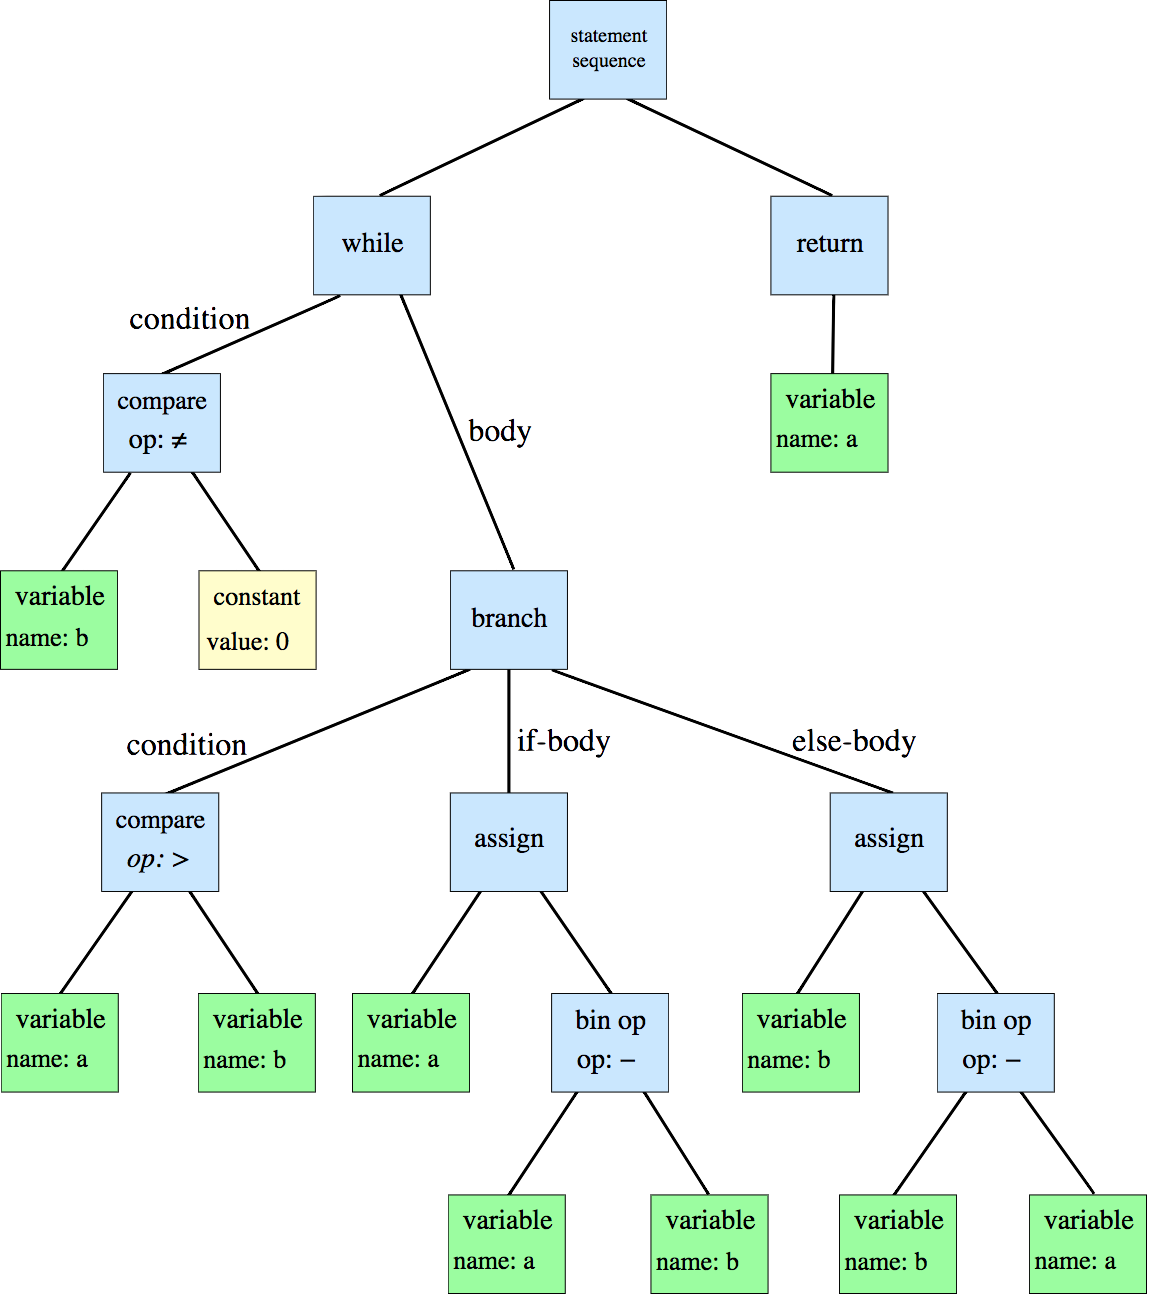
\includegraphics[width=6.0in]{./figures/Euclids_Greatest_Common_Divisor_Method.png}
  \end{center}}~\cite{DevlinetalICLR-18,WangetalCoRR-17};
% 
\end{itemize}

%%% %%%%%%%%%%%%%%%%%%%%%%%%%%%%%%%%%%%%%%%%%%%%%%%%%%%%%%%%%%%%%%%%%%%%%%%%%%%%
%%% %%%%%%%%%%%%%%%%%%%%%%%%%%%%%%%%%%%%%%%%%%%%%%%%%%%%%%%%%%%%%%%%%%%%%%%%%%%%

%%% PART II

%%% %%%%%%%%%%%%%%%%%%%%%%%%%%%%%%%%%%%%%%%%%%%%%%%%%%%%%%%%%%%%%%%%%%%%%%%%%%%%

\subsubsection*{PART II}

%%% %%%%%%%%%%%%%%%%%%%%%%%%%%%%%%%%%%%%%%%%%%%%%%%%%%%%%%%%%%%%%%%%%%%%%%%%%%%%

Referring to the abstractions and abbreviations introduced in the previous section, reading a program from {\tt{STDIO}} \emdash{} the analog of a human programmer reading a program displayed on a monitor \emdash{} will result in \emdash{} at least \emdash{} two different internal representations of the resulting AST: an embedding vector in the SMS and a key-value representation in the DNC. The former allows us manipulate programs and program fragments as fully-differentiable representations within distributed models. The latter allows us to modify, execute and share code in a human-accessible format, fully compatible with our software-development toolchain.

Following~\cite{PritzeletalICML-17}, we assume EMS consists of initial-state-action-reward-next-state tuples of the form $(s_{t},\;a_{t},\;r_{t},\;s_{t+1})$. State representations $s_{t}$ have to be detailed enough to reconstruct the context in which the action is performed and yet concise enough to be practical. Suppose the PFC directs the activation of selected circuits in the SMS via the GWS in accord with Dehaene~\etal{}~\cite{DehaeneetalSCIENCE-17,Dehaene2014} assuming a prior that generates low-dimensional thought vectors~\cite{BengioCoRR-17}. $s_{t}$ encodes the attentional state that served to identify representations in SMS relevant to $a_{t}$ allowing the EHC to produce the resulting state $s_{t+1}$. Given $s_{t}$ we can reproduce the activity recorded in the EMS, and, in principle, incorporate multiple steps and contingencies in a policy constituting a specialized program-synthesis or program-repair subroutine.

Such subroutines would include repairing a program in which a variable is introduced but not initialized, or when it is initialized but ambiguously typed or scoped. As another example, a variable is initialized as {\tt{VOID}} and subsequently assigned an integer value in some but not all branches of a conditional statement. Other examples of repair routines include problems with the use of comparison operators, e.g., conditional branches both with \hmleq{}, the {\tt{is}} operator is used instead of {\tt{is not}}, or vice versa, confusion involving {\tt{A is not None}}, {\tt{A not None}} and {\tt{A != None}}, and problems involving class methods, e.g., when {\tt{self}} accessor is missing from a variable, e.g., {\tt{mode = 'manual'}} instead of {\tt{self.mode = 'manual'}}~\cite{ShinetalICLR-18b,DevlinetalICLR-18,WangetalCoRR-17}.

Attentional machinery in the prefrontal cortex (PFC) populates the global workspace (GWS) by activating circuits relevant to the current input and internal state, including that of the DNC and any ongoing activity in (SMS) circuits produced by previous top-down attention and bottom-up sensory processing. The PFC in its role as executive arbiter identifies operators in the form of policy subroutines and then enlists the EHC to \emdash{} using terminology adapted from Von Neumann machines \emdash{} to load registers in short-term memory and perform operations by using fast weights to transform the contents of the loaded registers into product representations that can either be fed to associative embeddings, temporarily stored in other registers or used to modify the contents of the DNC thereby altering the AST representation of the target code and updating the display to provide feedback to the human programmer.

What's left out of this account so far includes how we might take advantage of semantics in the form of executing code and examining traces in order to better understand the consequences of the changes just made. Presumably, wrapping a code fragment in a function and executing the function with different input to examine changes in the state variables could be used as a distal reinforcement signal providing intermediate rewards useful in debugging subroutines. As pointed out earlier, subroutines designed to modify code are likely to involve many conditional choices and so it is important for subroutine policies to be highly conditioned on the status of specific state variables. Indeed a technique such as model-based parameter adaptation may be perfectly suited to providing such context-sensitive adaptations.

Perhaps this next thought seems obvious, but it is worth keeping in mind that the human brain does a great deal of (parallel) processing that never rises to the level of conscious attention. The executive control systems in the prefrontal cortex don't have micromanage everything. Every thought corresponds to a pattern of activity in one or more neural circuits in the brain or beyond in the peripheral nervous system. One pattern of activity inevitably leads to another in the same or another set of neurons. For example, patterns of activity that begin in the sensory cortex can lead to patterns of activity in the motor cortex and can have consequences elsewhere in the brain, e.g., in the cerebellar cortex resulting in speech, or external to the central nervous system as in the case of neurons that propagate through the peripheral nervous system causing muscles to contract and extend thereby making your limbs and torso move. 

Every new observation, every act of creating a new thought or revisiting an old one produces even more activity in the brain resulting in new thoughts some of which are ignored as their reverberations weaken and die and others that spawn new thoughts and proliferate under the influence of reentrant production of activity and the active encouragement of conscious attention in a perpetually self reinforcing, reimagining and self-analyzing cycle of recurrent activity. Meta-reinforcement learning supports the sort of diverse activity one might expect from a system that selects activity to attend to and then makes available in the global workspace for ready access by other systems. Sustaining a collection of such activated circuits would help to provide a context, serve to maintain a stack of policies, guide switching between them, support caching partial results for later use, reconstructing necessary state as needed when restoring policy after a recursive descent.

When you think of building systems that can develop new algorithms it is instructive the think about the simple case of learning to sort lists from input-output pairs. I would guess that bubble sort would be the easiest to come up with, but even then it is easier if you start with simple I/O pairs like $[A,\;B] \hmrarr{} [A,\;B], [B,\;A] \hmrarr{} [A,\;B]$ and work up to longer lists. As Dan Abolafia pointed out in his class {\urlh{https://web.stanford.edu/class/cs379c/calendar_invited_talks/lectures/04/24/index.html}{presentation}}, it is relative easy to learn to sort lists of length no more than $n$, but substantially more difficult to learn an algorithm that works for lists of arbitrary length, without the ability to construct a simple inductive proof of correctness. Logic and basic theorem proving are certainly important in learning to write programs. You might want to look at the Coq proof assistant\footnote{%
%
  {\urlh{https://en.wikipedia.org/wiki/Coq}{Coq}} is a formal proof management system that "provides a formal language to write mathematical definitions, executable algorithms and theorems together with an environment for semi-interactive development of machine-checked proofs" \emdash{} excerpted from Mike Nahas' {\urlh{https://coq.inria.fr/tutorial-nahas}{tutorial}}. The Coq formal language is also a programming language. It was developed by and named after its inventor, Thierry Coquand, and employed by Georges Gonthier and Benjamin Werner to create a new proof of the {\urlh{https://en.wikipedia.org/wiki/Four_color_theorem}{Four Color Theorem}} first proved by Kenneth Appel and Wolfgang Haken using a combination of human and computer theorem proving techniques.} for a glimpse at the future of algorithm development.

%%% %%%%%%%%%%%%%%%%%%%%%%%%%%%%%%%%%%%%%%%%%%%%%%%%%%%%%%%%%%%%%%%%%%%%%%%%%%%%
%%% %%%%%%%%%%%%%%%%%%%%%%%%%%%%%%%%%%%%%%%%%%%%%%%%%%%%%%%%%%%%%%%%%%%%%%%%%%%%

%%% PART III

%%% %%%%%%%%%%%%%%%%%%%%%%%%%%%%%%%%%%%%%%%%%%%%%%%%%%%%%%%%%%%%%%%%%%%%%%%%%%%% 

\subsubsection*{PART III}

%%% %%%%%%%%%%%%%%%%%%%%%%%%%%%%%%%%%%%%%%%%%%%%%%%%%%%%%%%%%%%%%%%%%%%%%%%%%%%% 

\setcounter{figure}{0}

%%% %%%%%%%%%%%%%%%%%%%%%%%%%%%%%%%%%%%%%%%%%%%%%%%%%%%%%%%%%%%%%%%%%%%%%%%%%%%% 

%%% Figure~{\urlh{#fig_Integrated_Architecture_Integrated_Figure}{1}}
\rawhtml
<a name="fig_Integrated_Architecture_Integrated_Figure"></a>
\endrawhtml
\begin{figure}
%
  \hrule{}
%
  \begin{center}
    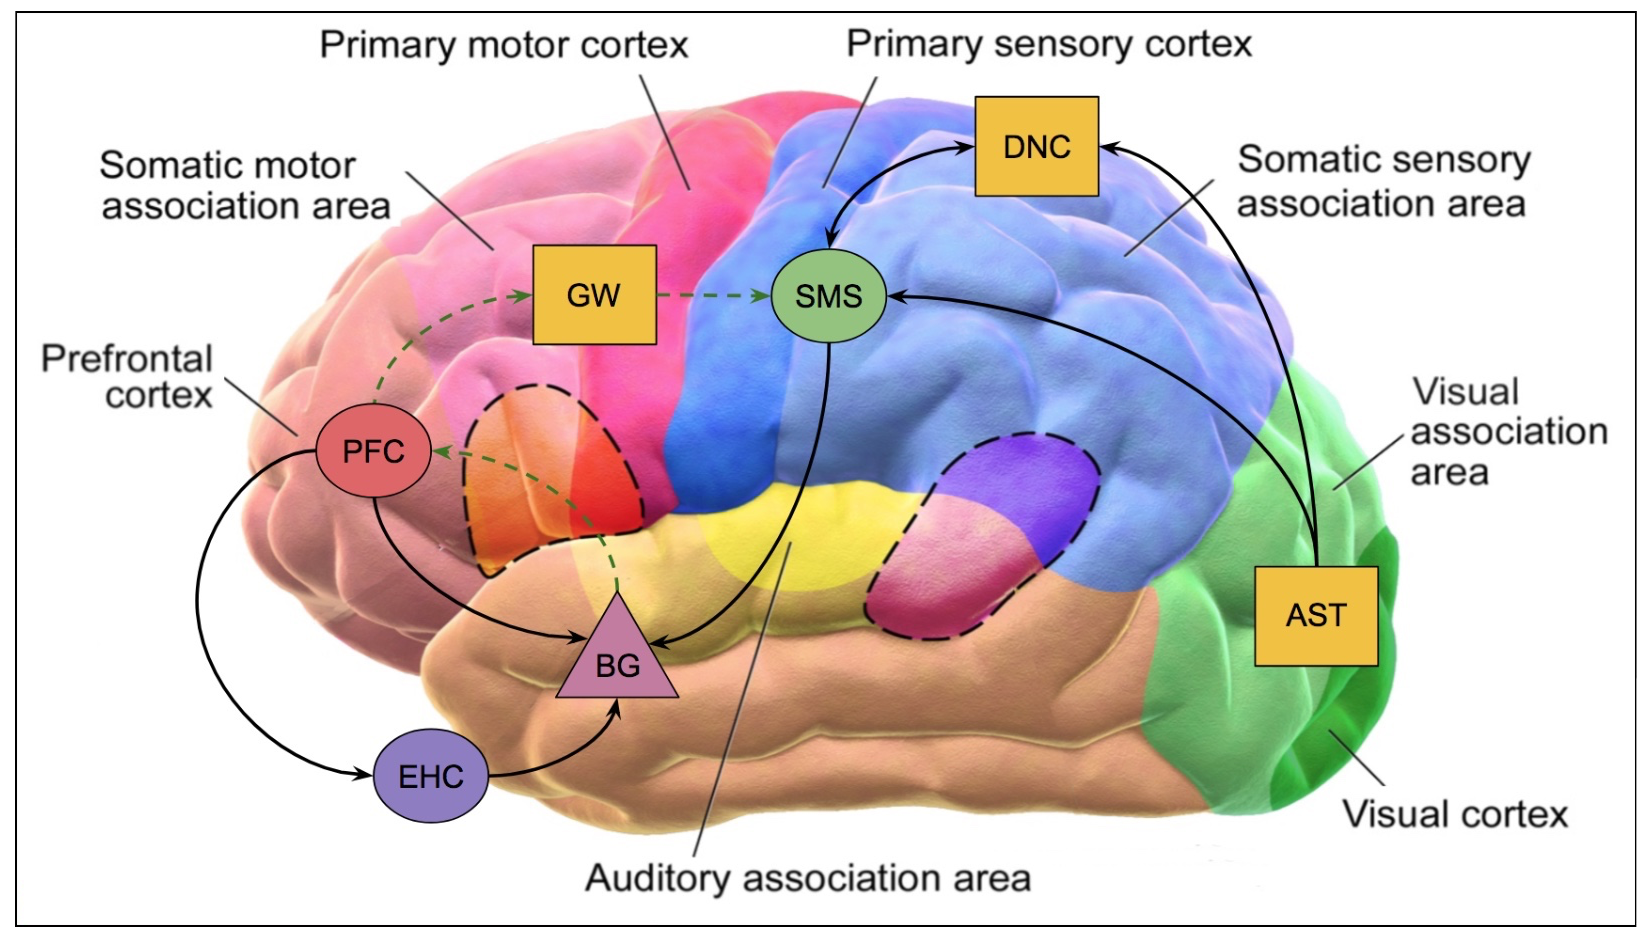
\includegraphics[width=11.0in]{./figures/Integrated_Architecture_Integrated_Figure.png}
  \end{center}
%
  \caption{The triptych on the bottom concatenates the graphics from three papers by Randal O'Reilly and his colleagues. They are reproduced here along with their original captions for your convenience in understanding the graphic in the top panel labeled {\rawhtml<span style="color:red">(a)</span>\endrawhtml} that is explained in detail in the main text. Panel {\rawhtml<span style="color:red">(a)</span>\endrawhtml} follows the shape and color conventions employed in Panel {\rawhtml<span style="color:red">(c)</span>\endrawhtml} except the yellow square shapes that denote abstract structures and not anatomical features. The acronyms are expanded and explained {\urlh{#convention_and_abbreviation_index}{here}}.
    %%% OReillySCIENCE-06_Figure_02_Dynamic.png
    Figure~2 in O'Reilly~\cite{OReillySCIENCE-06} shown in Panel {\rawhtml<span style="color:red">(b)</span>\endrawhtml} \emdash{} Dynamic gating produced by disinhibitory circuits through the basal ganglia and frontal cortex/PFC (one of multiple parallel circuits shown).  In the base state (no striatum activity) and when {\tt{NoGo}} (indirect pathway) striatum neurons are firing more than {\tt{Go}}, the SNr (substantia nigra pars reticulata) is tonically active and inhibits excitatory loops through the basal ganglia and PFC through the thalamus. This corresponds to the gate being closed, and PFC continues to robustly maintain ongoing activity (which does not match the activity pattern in the posterior cortex, as indicated). When direct pathway {\tt{Go}} neurons in striatum fire, they inhibit the SNr and thus disinhibit the excitatory loops through the thalamus and the frontal cortex, producing a gating-like modulation that triggers the update of working memory representations in prefrontal cortex. This corresponds to the gate being open.
    %%% OReillyetalLEABRA-16_Figure_07_Leabra.png
    Figure~7 in O'Reilly~\etal{}~\cite{OReillyetalLEABRA-16} shown in Panel {\rawhtml<span style="color:red">(c)</span>\endrawhtml} \emdash{} The macrostructure of the {\urlh{https://en.wikipedia.org/wiki/Leabra}{Leabra}} architecture, with specialized brain areas interacting to produce overall cognitive function.
    %%% OReillyetalLEABRA-16_Figure_08_Leabra.png
    Figure~8 in O'Reilly~\etal{}~\cite{OReillyetalLEABRA-16} shown in Panel {\rawhtml<span style="color:red">(d)</span>\endrawhtml} \emdash{} Structure of the hippocampal memory system and associated medial temporal lobe cortical structures including entorhinal cortex.}
%
  \hrule{}
%
\end{figure}

%%% %%%%%%%%%%%%%%%%%%%%%%%%%%%%%%%%%%%%%%%%%%%%%%%%%%%%%%%%%%%%%%%%%%%%%%%%%%%% 

Figure~{\urlh{#fig_Integrated_Architecture_Integrated_Figure}{1}} shows a diagram of the human brain overlaid with a simplified architectural drawing. The box shapes represent abstract systems and the oval and triangular shapes represent anatomical features for which we can supply computational models. For example, the box labeled GW represents the global workspace which performs particular function in the architecture, but actually spans a good portion of the neocortex. Whereas the triangle labeled BG represents a group of subcortical nuclei called the basal ganglia situated at the base of the forebrain.

The box labeled AST represents a form of sensory input corresponding to the ingestion of abstract syntax trees representing code fragments. The oval labeled SMS represents semantic memory and the box labeled DNC corresponds to a differentiable neural computer. When the system ingests a new program fragment the resulting AST is encoded in the SMS as an embedding vector and simultaneously as a set of key-value pairs in the DNC. Here we think of the DNC as a body part or external prosthesis with corresponding maps in the somatosensory and motor cortex that enable reading and writing respectively.

Our explanation of the architecture proceeds top down, as it were, with a discussion of executive function in the prefrontal cortex. The GWS provides two-way connection between structures in the prefrontal cortex and homologous structures of a roughly semantic character throughout the rest of neocortex thereby enabling the PFC to listen in on diverse circuits in the neocortex and select a subset of such circuits for attention. Stanislas Dehaene describes this process as the function of consciousness, but we need not commit ourselves to such interpretation here.

Not only does the PFC selectively activate circuits but it can also maintain the activity such circuits indefinitely as constituents of working memory. Since this capability is limited by the capacity of the PFC, the content of working memory is limited and adding new constituents may curtail the activation of existing constituents. In practice, we intend to model this capability using meta-reinforcement learning~\cite{WangetalNATURE-NEUROSCIENCE-18} (MRL) in which the MRL system relies on the GWS network to sample, evaluate and select constitute circuits guided by a suitable prior~\cite{BengioCoRR-17} and past experience and then maintain their activity by a combination of memory networks~\cite{WestonetalCoRR-14} and fast weights~\cite{BaetalCoRR-16}. 

%%% %%%%%%%%%%%%%%%%%%%%%%%%%%%%%%%%%%%%%%%%%%%%%%%%%%%%%%%%%%%%%%%%%%%%%%%%%%%% 

Meta-reinforcement learning serves a second complementary role in the PFC related to executive function. We will refer to the first role as MRL-A for "attention" and the second as MRL-P for "planning". MRL-A is trained to focus attention on relevant new sensory input and new interpretations of and associations among prior perceptions and thoughts. MRL-P is trained to capitalize on and respond to opportunities made available by new and existing constituents in working memory. Essentially MRL-P is responsible for the scheduling and deployment of plans relevant to recognized opportunities to act. These plans are realized as policies trained by reinforcement learning from traces of past experience or constructed on the fly in response to unexpected / unfamiliar contingencies by recovering and reimagining past activities recovered from episodic memory.

MRL-A and MRL-P could be implemented as a single policy, but it is simpler to think of them as two coupled systems, one responsible for focusing attention by constantly assessing changes in (neural) activity throughout the global workspace, and a second responsible for overseeing the execution of plans in responding to new opportunities to solve problems. MRL-A is as a relatively straightforward reinforcement learning system independently performing its task largely a function of whatever neural activity is going on in the GW, its attentional network and the prior baked into its reward function. MRL-P could be implemented along the lines of the Imagination-Augmented Agent (I2A) architecture~\cite{WeberetalCoRR-17} or the related Imagination-Based Optimization~\cite{HamricketalCoRR-17} and Imagination-Based Planning~\cite{PascanuetalCoRR-17} systems.

%%% %%%%%%%%%%%%%%%%%%%%%%%%%%%%%%%%%%%%%%%%%%%%%%%%%%%%%%%%%%%%%%%%%%%%%%%%%%%%

The remaining parts of the architecture involve the interplay between the PFC and the semantic and episodic memory systems as facilitated by the basal ganglia and hippocampus. If we had a policy pre-trained for every possible contingency, we would be nearly done \emdash{} let MRL-A draw attention to relevant internal and external activity and then design a simple just-in-time greedy scheduler that picks the policy with the highest reward given the state vector corresponding to the current content of working memory. Unfortunately, the life of an apprentice programmer is not nearly so simple.

The apprentice might listen to advice from a human programmer or watch someone solve a novel coding problem or repair a buggy program. Alternatively, it may be relatively simple to adapt an existing policy to work in the present circumstances. However, making progress on harder problems will depend on expert feedback or having an existing reward function that generalizes to the problem at hand. In the remainder of this entry, we set aside these problems for another day and concentrate on the basic functionality provided by the basal ganglia as highlighted in Panel {\rawhtml<span style="color:red">(c)</span>\endrawhtml} \emdash{} of Figure~{\urlh{#fig_Integrated_Architecture_Integrated_Figure}{1}}.

The basal ganglia in cognitive models such as the one described by Randall O'Reilly's in his {\urlh{https://web.stanford.edu/class/cs379c/calendar_invited_talks/lectures/04/12/index.html}{presentation}} in class, play a central role in action selection. This seems like a good opportunity to review how actions are represented in deep-neural-network implementations of reinforcement learning. Returning to our default representation for the simplest sort of episodic memory, $(s_{t},\;a_{t},\;r_{t},\;s_{t+1})$, it’s easy to think of a state $s$ as a vector $s \hmisin{} \hmreals{}^{n}$ and a reward $r$ as a scalar value, $r \hmisin{} \hmreals{}$, but how are actions represented?

Most approaches to deep reinforcement learning employ a tablular model of the policy implying a finite \emdash{} and generally rather small \emdash{} repertoire of actions. For example, most of the experiments described in Wayne~\etal{}~\cite{WayneetalCoRR-18} (MERLIN) six-dimensional one-hot binary vector that maps a set of six actions: move forward, move backward, rotate left with rotation rate of 30, rotate right with rotation rate of 30, move forward and turn left, move forward and turn right. The action space for the grid-world problems described in Rabinowitz~\etal{}~\cite{RabinowitzetalCoRR-18} (ToMnets) consists of four movement actions: up, down, left, right and stay.

%%% %%%%%%%%%%%%%%%%%%%%%%%%%%%%%%%%%%%%%%%%%%%%%%%%%%%%%%%%%%%%%%%%%%%%%%%%%%%%
%%% %%%%%%%%%%%%%%%%%%%%%%%%%%%%%%%%%%%%%%%%%%%%%%%%%%%%%%%%%%%%%%%%%%%%%%%%%%%%

%%% PART IV

%%% %%%%%%%%%%%%%%%%%%%%%%%%%%%%%%%%%%%%%%%%%%%%%%%%%%%%%%%%%%%%%%%%%%%%%%%%%%%%

\subsubsection*{PART IV}

%%% %%%%%%%%%%%%%%%%%%%%%%%%%%%%%%%%%%%%%%%%%%%%%%%%%%%%%%%%%%%%%%%%%%%%%%%%%%%%

The programmer's apprentice (PA) operates on programs represented as trees, where the set of actions includes basic operations for traversing and editing trees \emdash{} or more generally directed-graphs with cycles if you assume edges in abstract syntax trees corresponding to loops, recursion and nested procedure calls, i.e., features common to nearly all the programs we actually care about. We still have a finite number of actions since for any given project we can represent the code base as a directed-acylic graph with annotations to accommodate procedure calls and recursion, and use attention to direct and contextualize a finite set of edit operations\footnote{%
%
  While the apprentice operates directly on the AST representation of the code, the IDE can be designed to periodically coerce this representation into a syntactically-correct form, display the result as human-readable code, and display meaningful annotations that highlight program fragments relevant to the ongoing collaboration and track the apprentice's attention.}.

Pritzel~\etal{}~\cite{PritzeletalCoRR-17} employ a semi-tabular representation of an agent's experience of the environment possessing features of episodic memory including long-term memory, sequentiality and context-based lookups. The representation called a {\it{differential neural dictionary}} (DND) is related to Graves~\etal{}~\cite{GravesetalNATURE-16} DNC. The programmer's apprentice is better suited to Vinyals~\etal{}~\cite{VinyalsetalNIPS-15} related idea of a {\it{pointer-network}} designed to learn the conditional probability of an output sequence with elements that are discrete tokens corresponding to positions in an input sequence \emdash{} see related work in natural language processing by Merity~\etal{}~\cite{MerityetalCoRR-16} on {\it{pointer sentinels}}.

%%% %%%%%%%%%%%%%%%%%%%%%%%%%%%%%%%%%%%%%%%%%%%%%%%%%%%%%%%%%%%%%%%%%%%%%%%%%%%% 

\setcounter{figure}{1}

%%% %%%%%%%%%%%%%%%%%%%%%%%%%%%%%%%%%%%%%%%%%%%%%%%%%%%%%%%%%%%%%%%%%%%%%%%%%%%% 

%%% Figure~{\urlh{#fig_SeeetalACL-17_Figure_03}{2}}
\rawhtml
<a name="fig_SeeetalACL-17_Figure_03"></a>
\endrawhtml
\begin{figure}
%
  \hrule{}
%
  \begin{center}
    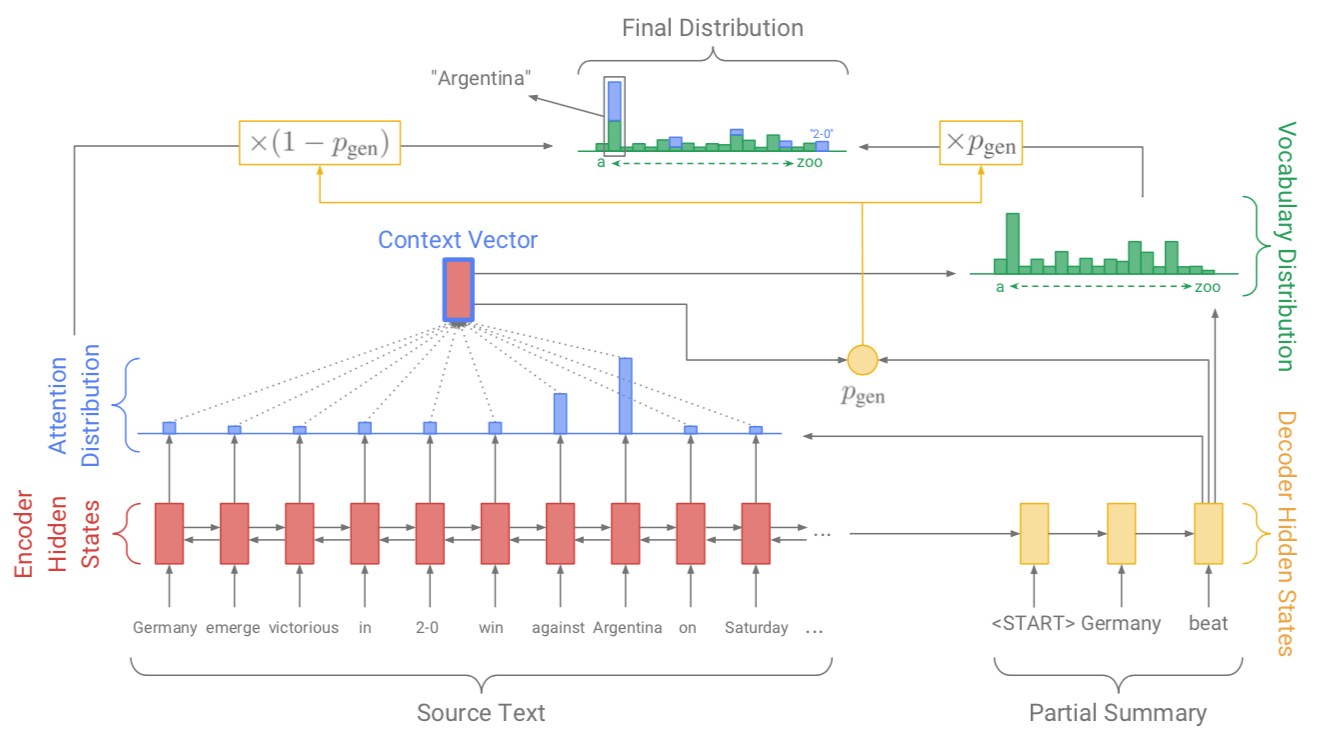
\includegraphics[width=11.0in]{./figures/SeeetalACL-17_Figure_03.png}
  \end{center}
%
  \caption{Pointer-generator model. For each decoder timestep a generation probability $P\mbox{\rm{gen}} \hmisin{} [0, 1]$ is calculated, which weights the probability of {\it{generating}} words from the vocabulary, versus {\it{copying}} words from the source text. The vocabulary distribution and the attention distribution are weighted and summed to obtain the final distribution, from which we make our prediction. Note that out-of-vocabulary article words such as 2-0 are included in the final distribution. \emdash{} adapted from~\cite{SeeetalACL-17}.}
%
  \hrule{}
%
\end{figure}

%%% %%%%%%%%%%%%%%%%%%%%%%%%%%%%%%%%%%%%%%%%%%%%%%%%%%%%%%%%%%%%%%%%%%%%%%%%%%%% 

\rawhtml
<a name="automated_programming_code_repair"></a>
\endrawhtml

One approach involves representing a program as an abstract syntax tree and performing a series of repairs that involve replacing complete subtrees in the AST. It might be feasible to use some variant of the pointer-network concept, e.g., {\cite{BhoopchandetalICLR-17}}, {\cite{SeeetalACL-17}} and  {\cite{WangandJiangICLR-17}} or neural programmer framework {\cite{NeelakantanetalICLR-17}}, but there are limitations with all of the alternatives I've run across so far, requiring additional innovation to deal with the dynamic character of editing AST representations, but at least the parsing problem is solved for us \emdash{} all we have to do is make sure that our edits maintain syntactic well-formedness.

Most of the existing pointer-network applications analyze / operate on a fixed structure such as a road map, e.g., examples include the planar graphs that Oriol Vinyals addresses in his paper~\cite{VinyalsetalNIPS-15}, recognizing long-range dependencies in code repositories~\cite{BhoopchandetalICLR-17}, and annotating text to support summarization~\cite{SeeetalACL-17}. Student projects focusing on program-repair might try ingesting programs using an LSTM, creating a pointer-network / DNC-like representation of the AST and then altering selected programs by using fragments from other programs, but be advised this approach will likely require inventing extensions to existing pointer-network techniques.

One possibility for training data is to use the ETH / SRI Python {\urlh{https://www.sri.inf.ethz.ch/py150}{dataset}} that was developed by Veselin Raychev as part of his {\urlh{https://www.sri.inf.ethz.ch/raychev_thesis.pdf}{thesis}} on automated code synthesis\footnote{%
%
  From the ETH/SRI website: "We provide a dataset consisting of parsed Parsed ASTs that were used to train and evaluate the DeepSyn tool. The Python programs are collected from GitHub repositories by removing duplicate files, removing project forks (copy of another existing repository), keeping only programs that parse and have at most 30K nodes in the AST and we aim to remove obfuscated files. Furthermore, we only used repositories with permissive and non-viral licenses such as MIT, BSD and Apache. For parsing, we used the Python AST parser included in Python 2.7. We also include the parser as part of our dataset. The dataset is split into two parts \emdash{} 100K files used for training and 50K files used for evaluation."}.
%
Possible projects include designing a rewrite system for code synthesis based on NLP work from Chris Manning's lab led by Abigail See~\cite{SeeetalACL-17} focusing on text summarization leveraging pointer networks \emdash{} see Figure~{\urlh{#fig_SeeetalACL-17_Figure_03}{2}} for an excellent schematic overview of their method. Further afield are program synthesis papers that work starting from specifications like Shin~\etal{}~\cite{ShinetalICLR-18b} out of Dawn Song's lab or recent work from Rishabh Singh and his colleagues~\cite{WangetalCoRR-17}.

Another possibility is to use RL to learn repair rules that operate directly on the AST using various strategies. It's not necessary in this case to represent the AST as a pointer network, but, rather, take the expedient of simply creating a new embedding edited AST after each repair. We can generate synthetic data by taking correct programs from the ETH/SRI dataset and introducing bugs and then use these to generate a reward signal, with harder problems requiring two or three separate repairs. 

It might also be worth exploring the idea of working with program embedding vectors in a manner similar to performing arithmetic operations on word vectors in order to recover analogies \emdash{} see the analysis of Levy and Goldberg~\cite{LevyandGoldbergCONIL-14} in which they demonstrate that analogy recovery is not restricted to simple neural word embeddings. For example, given the AST for a program {\tt{P}} with subtree {\tt{Q}} and two possible repairs that correspond to replacing {\tt{Q}} with either {\tt{R}} or {\tt{R'}}, can we determine which is the better outcome {\tt{A = P - Q + R}} or {\tt{A' = P - Q + R'}} and might it serve as a distal reward signal to expedite training?

I also recommend Reed and de Freitas~\cite{ReedandDeFreitasCoRR-15} for its application of the idea of using dynamically programmable networks in which the activations of one network become the weights (program) of another network.  The authors note that this approach was mentioned in Sigma-Pi units section of Rumelhart~\etal{}~\cite{RumelhartetalPDP-86b}, appeared in Sutskever and Hinton~\cite{SutskeverandHintonNIPS-09} in the context of learning higher order symbolic relations and in Donnarumma~\etal{}~\cite{DonnarummaetalIJNS-15} as the key ingredient of an architecture for prefrontal cognitive control.

%%% %%%%%%%%%%%%%%%%%%%%%%%%%%%%%%%%%%%%%%%%%%%%%%%%%%%%%%%%%%%%%%%%%%%%%%%%%%%%
%%% %%%%%%%%%%%%%%%%%%%%%%%%%%%%%%%%%%%%%%%%%%%%%%%%%%%%%%%%%%%%%%%%%%%%%%%%%%%%


